\documentclass[11pt,a4paper]{article}
\usepackage[T1]{fontenc}
\usepackage[utf8]{inputenc}
\usepackage{lmodern}
\usepackage{textcomp}
\usepackage[left=1.8cm,right=1.8cm,top=2.3cm,bottom=2.2cm,headheight=14pt,headsep=8pt]{geometry}
\usepackage{multicol}
\usepackage{xcolor}
\usepackage{fancyhdr}
\usepackage{graphicx}
\usepackage{array}
\usepackage{amsmath,amssymb}
\usepackage{setspace}
\usepackage{longtable}
\graphicspath{{../}}
\definecolor{ygreen}{RGB}{46,139,87}
\renewcommand{\normalsize}{\fontsize{10.9}{13.4}\selectfont}
\renewcommand{\familydefault}{\rmdefault}
\setlength{\parindent}{0pt}
\setlength{\columnsep}{0.8cm}
\setlength{\columnseprule}{0.4pt}
\setlength{\multicolsep}{3pt plus 1pt minus 1pt}
\renewcommand{\textsubscript}[1]{\ensuremath{_{\text{\fontsize{8}{8}\selectfont #1}}}}
\renewcommand{\textsuperscript}[1]{\ensuremath{^{\text{\fontsize{8}{8}\selectfont #1}}}}
\newcommand{\diqqat}[1]{\par\smallskip\noindent\textbf{Diqqat!} #1\par\medskip}
\newcommand{\javob}{\par\smallskip\noindent\textbf{Javob:} \rule[-2pt]{7.5cm}{0.4pt}\par\smallskip\noindent\textbf{Diqqat!} Javobingizni javoblar varaqasiga ko`chirib yozing.\par\medskip}
\pagestyle{fancy}
\fancyhf{}
\renewcommand{\headrulewidth}{0.4pt}
\fancyhead[L]{\textit{Milliy sertifikat 2026. Kimyo}}
\fancyhead[R]{6-variant}
\fancyfoot[L]{\fontsize{8}{9}\selectfont \textcopyright{} Colba maktabi, 2026}
\fancyfoot[C]{\thepage}
\fancypagestyle{first}{\fancyhf{}\renewcommand{\headrulewidth}{0pt}\fancyfoot[L]{\fontsize{8}{9}\selectfont \textcopyright{} Colba maktabi, 2026}\fancyfoot[C]{\thepage}}
\begin{document}
\normalsize
\thispagestyle{first}
\noindent\fcolorbox{ygreen}{white}{\parbox{\dimexpr\linewidth-2\fboxsep-2\fboxrule\relax}{%
\textbf{\fontsize{13}{15}\selectfont Nazorat testi}\ \textit{\fontsize{10}{12}\selectfont $\cdot$ Aralash test $\cdot$ 6-variant}\hfill
\begin{tabular}[t]{@{}r@{}}\textit{Milliy sertifikat 2026. Kimyo}\\ \textbf{\textit{\fontsize{8}{9}\selectfont Vaqt:}} \textit{\fontsize{10}{12}\selectfont 180 daqiqa}\end{tabular}}}
\par\medskip
\noindent\textit{Davriy jadvaldan foydalanish mumkin.}
\par\medskip
\begin{multicols}{2}
\noindent\textbf{1.} Quyidagi moddalarning qaysilarida ion bog` mavjud? 1) (NH\textsubscript{4})\textsubscript{2}SO\textsubscript{4}; 2) NH\textsubscript{4}Cl; 3) H\textsubscript{2}O; 4) NaCl

\noindent A)~\textsl{1, 2, 3} \hfill B)~\textsl{3, 4} \hfill C)~\textsl{1, 2, 4} \hfill D)~\textsl{1, 3}\par
\vspace{4pt}
\noindent\textbf{2.} 10 l N\textsubscript{2} va 45 l H\textsubscript{2} aralashmasi reaksiyaga kirishdi (N\textsubscript{2} + 3H\textsubscript{2} $\to$ 2NH\textsubscript{3}, hamma moddalar bir xil sharoitda gaz holida). Reaksiyadan keyingi gaz aralashmasining \textbf{hajmini (l) aniqlang.}

\noindent A)~\textsl{55} \hfill B)~\textsl{20} \hfill C)~\textsl{15} \hfill D)~\textsl{35}\par
\vspace{4pt}
\noindent\textbf{3.} Reaksiyaning energetik diagrammasi berilgan (boshlang`ich moddalar energiyasi 20, mahsulotlar 90 kJ/mol).
\begin{center}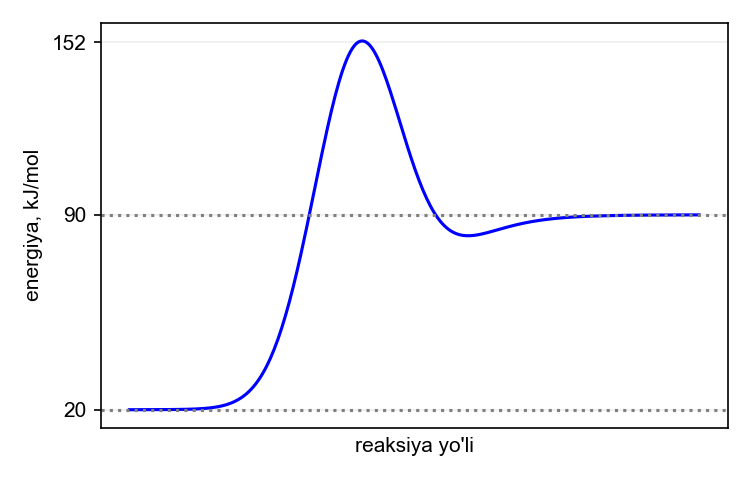
\includegraphics[width=0.86\linewidth]{rasmlar/gen/en_v06_0.png}\end{center}
Reaksiya qaysi turga kiradi?

\noindent\begin{tabular}{@{}p{0.47\linewidth}@{}p{0.47\linewidth}@{}}
A)~\textsl{endotermik} & B)~\textsl{ekzotermik} \\
C)~\textsl{katalitik} & D)~\textsl{teskarilanmas} \\
\end{tabular}\par
\vspace{4pt}
\noindent\textbf{4.} CH\textsubscript{2}=CH--CH=CH\textsubscript{2} molekulasidagi $\sigma$ va $\pi$ bog`lar \textbf{sonini aniqlang.}

\noindent A)~\textsl{8 va 2} \hfill B)~\textsl{9 va 3} \hfill C)~\textsl{10 va 2} \hfill D)~\textsl{9 va 2}\par
\vspace{4pt}
\noindent\textbf{5.} Jadvalda Cl elementining birikmalaridagi oksidlanish darajasi berilgan:
\begin{center}
\renewcommand{\arraystretch}{1.15}
\begin{tabular}{|c|c|}\hline
\textbf{Modda} & \textbf{Oksidlanish darajasi} \\ \hline
KClO\textsubscript{3} & +5 \\ \hline
HCl & -1 \\ \hline
NaCl & -1 \\ \hline
HClO & +1 \\ \hline
\end{tabular}
\end{center}
Ushbu moddalardan nechtasida Cl elementi ham oksidlovchi, ham qaytaruvchi xossani namoyon qiladi? (Cl uchun eng past oksidlanish darajasi -1, eng yuqorisi +7)

\noindent A)~\textsl{3} \hfill B)~\textsl{2} \hfill C)~\textsl{4} \hfill D)~\textsl{5}\par
\vspace{4pt}
\noindent\textbf{6.} 40 l H\textsubscript{2}S va 180 l O\textsubscript{2} aralashmasi 2H\textsubscript{2}S + 3O\textsubscript{2} $\to$ 2SO\textsubscript{2} + 2H\textsubscript{2}O tenglama bo`yicha to`liq reaksiyaga kirishdi (reaksiyadan so`ng suv suyuq holatda; gazlar bir xil sharoitda o`lchandi). Reaksiyadan so`ng hosil bo`lgan gazlar aralashmasining umumiy \textbf{hajmini (l) aniqlang.}

\noindent A)~\textsl{220} \hfill B)~\textsl{160} \hfill C)~\textsl{40} \hfill D)~\textsl{120}\par
\vspace{4pt}
\noindent\textbf{7.} Na\textsubscript{2}SO\textsubscript{4} ning suvli eritmasi inert elektrodlar bilan elektroliz qilinganda qaysi moddalar ajraladi?

\noindent\begin{tabular}{@{}p{0.47\linewidth}@{}p{0.47\linewidth}@{}}
A)~\textsl{H\textsubscript{2} va O\textsubscript{2}} & B)~\textsl{H\textsubscript{2}, Cl\textsubscript{2} va NaOH} \\
C)~\textsl{Cu va Cl\textsubscript{2}} & D)~\textsl{Ag va O\textsubscript{2}} \\
\end{tabular}\par
\vspace{4pt}
\noindent\textbf{8.} Rasmda molekulaning sharsimon modeli tasvirlangan (qora -- C, qizil -- O, ko`k -- N, oq -- H).
\begin{center}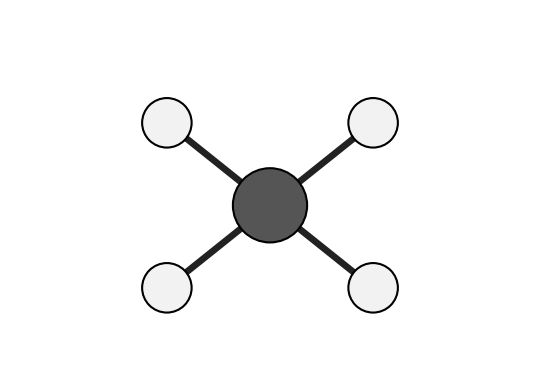
\includegraphics[width=0.86\linewidth]{rasmlar/gen/md_697606.png}\end{center}
Molekuladagi $\pi$-bog`lar \textbf{sonini aniqlang.}

\noindent A)~\textsl{1} \hfill B)~\textsl{0} \hfill C)~\textsl{2} \hfill D)~\textsl{3}\par
\vspace{4pt}
\noindent\textbf{9.} Jadvalda metall plastinkalarning tuz eritmalariga tushirilishidagi kuzatuvlar berilgan (``+'' -- metall ajraladi, reaksiya boradi; ``$-$'' -- reaksiya bormaydi):
\begin{center}
\renewcommand{\arraystretch}{1.15}
\begin{tabular}{|c|c|c|c|}\hline
\textbf{Metall} & \textbf{CuSO\textsubscript{4} eritmasi} & \textbf{ZnSO\textsubscript{4} eritmasi} & \textbf{FeSO\textsubscript{4} eritmasi} \\ \hline
Zn & + & $-$ & + \\ \hline
Mg & + & + & + \\ \hline
Cu & $-$ & $-$ & $-$ \\ \hline
\end{tabular}
\end{center}
Ushbu metallardan qaysi biri eng faol?

\noindent A)~\textsl{Zn} \hfill B)~\textsl{Cu} \hfill C)~\textsl{Fe} \hfill D)~\textsl{Mg}\par
\vspace{4pt}
\noindent\textbf{10.} 4,8 g metall kislotada eritilganda 4,48 l (n.sh.) vodorod ajraldi. Metallning ekvivalent \textbf{massasini (g/mol) aniqlang} (\textit{V}\_E(H\textsubscript{2}) = 11,2 l/mol).

\noindent A)~\textsl{24} \hfill B)~\textsl{6} \hfill C)~\textsl{53,76} \hfill D)~\textsl{12}\par
\vspace{4pt}
\noindent\textbf{11.} Quyidagi zarrachalardan qaysilari neon atomi bilan izoelektron? 1) Na\textsuperscript{+}; 2) Li\textsuperscript{+}; 3) Mg\textsuperscript{2+}; 4) F\textsuperscript{$-$}

\noindent A)~\textsl{1, 2, 4} \hfill B)~\textsl{1, 2} \hfill C)~\textsl{1, 2, 3} \hfill D)~\textsl{1, 3, 4}\par
\vspace{4pt}
\noindent\textbf{12.} Oltingugurt (\textit{Z} = 16) atomining tashqi energetik pog`onasidagi elektronlar \textbf{sonini aniqlang.}

\noindent A)~\textsl{7} \hfill B)~\textsl{6} \hfill C)~\textsl{5} \hfill D)~\textsl{8}\par
\vspace{4pt}
\noindent\textbf{13.} Hajmi 5 l bo`lgan idishda A modda miqdori 100 s davomida 1,2 mol ga kamaydi. Reaksiyaning o`rtacha tezligini (mol/(l$\cdot$s)) \textbf{toping.}

\noindent A)~\textsl{0,0024} \hfill B)~\textsl{0,012} \hfill C)~\textsl{0,24} \hfill D)~\textsl{0,06}\par
\vspace{4pt}
\noindent\textbf{14.} Qaysi juftliklar o`zaro reaksiyaga kirishadi? 1) SiO\textsubscript{2} va H\textsubscript{2}O; 2) Ag va H\textsubscript{2}SO\textsubscript{4}(suyult.); 3) MgCl\textsubscript{2} va KNO\textsubscript{3}; 4) Fe va HCl

\noindent A)~\textsl{2, 3} \hfill B)~\textsl{1} \hfill C)~\textsl{4} \hfill D)~\textsl{3, 4}\par
\vspace{4pt}
\noindent\textbf{15.} 37,8 g Zn(NO\textsubscript{3})\textsubscript{2} to`liq parchalanguncha qizdirildi. Qattiq qoldiq \textbf{massasini (g) aniqlang.}

\noindent A)~\textsl{37,8} \hfill B)~\textsl{32,4} \hfill C)~\textsl{16,2} \hfill D)~\textsl{8,1}\par
\vspace{4pt}
\noindent\textbf{16.} 0,2 mol NaOH tutgan eritmadan 0,15 mol CO\textsubscript{2} o`tkazildi. Hosil bo`lgan NaHCO\textsubscript{3} \textbf{massasini (g) aniqlang.}

\noindent A)~\textsl{8,4} \hfill B)~\textsl{2,1} \hfill C)~\textsl{8} \hfill D)~\textsl{4,2}\par
\vspace{4pt}
\noindent\textbf{17.} Reaksiya tenglamasi: 2NaCl + H\textsubscript{2}SO\textsubscript{4} $\to$ Na\textsubscript{2}SO\textsubscript{4} + 2HCl. Reaksiyaga 196 g H\textsubscript{2}SO\textsubscript{4} kirishdi. HCl \textbf{massasini (g) hisoblang.}

\noindent A)~\textsl{146} \hfill B)~\textsl{36,5} \hfill C)~\textsl{292} \hfill D)~\textsl{73}\par
\vspace{4pt}
\noindent\textbf{18.} Li va K dan iborat 6 g aralashma suv bilan reaksiyaga kirishdi. Ajralgan vodorodning \textbf{hajmini (l, n.sh.) aniqlang.}

\noindent A)~\textsl{8,96} \hfill B)~\textsl{2,24} \hfill C)~\textsl{4,48} \hfill D)~\textsl{3}\par
\vspace{4pt}
\noindent\textbf{19.} Alyuminiy (0,2 mol) va magniy (0,2 mol) aralashmasi mo`l xlorid kislotada eritildi. Ajralgan vodorodning \textbf{hajmini (l, n.sh.) aniqlang.}

\noindent A)~\textsl{11,2} \hfill B)~\textsl{8,96} \hfill C)~\textsl{22,4} \hfill D)~\textsl{5,6}\par
\vspace{4pt}
\noindent\textbf{20.} CH\textsubscript{3}--C(CH\textsubscript{3})\textsubscript{2}--OH birikmaning sistematik nomi qaysi qatorda to`g`ri keltirilgan?

\noindent\begin{tabular}{@{}p{0.47\linewidth}@{}p{0.47\linewidth}@{}}
A)~\textsl{butanol-2} & B)~\textsl{2-metilpropanol-1} \\
C)~\textsl{2-metilpropanol-2} & D)~\textsl{butanol-1} \\
\end{tabular}\par
\vspace{4pt}
\noindent\textbf{21.} Alken, alkadiyen va alkinlar haqida qaysi fikrlar to`g`ri? 1) Etilen bromli suvni rangsizlantiradi; 2) Kauchuk izoprenning polimeri; 3) Alkenlar KMnO\textsubscript{4} ning suvli eritmasi bilan glikol hosil qiladi; 4) Propenga HBr birikishi Markovnikov qoidasiga bo`ysunadi

\noindent\begin{tabular}{@{}p{0.47\linewidth}@{}p{0.47\linewidth}@{}}
A)~\textsl{1, 2, 4} & B)~\textsl{1, 3, 4} \\
C)~\textsl{1, 2, 3, 4} & D)~\textsl{1, 2, 3} \\
\end{tabular}\par
\vspace{4pt}
\noindent\textbf{22.} 0,6 mol asetilendan Zelinskiy usuli bilan (80\% unum) benzol olindi. Benzol \textbf{massasini (g) aniqlang.}

\noindent A)~\textsl{12,48} \hfill B)~\textsl{37,44} \hfill C)~\textsl{15,6} \hfill D)~\textsl{5,2}\par
\vspace{4pt}
\noindent\textbf{23.} C\textsubscript{6}H\textsubscript{12}O\textsubscript{6} $\to$ 2C\textsubscript{2}H\textsubscript{5}OH + 2CO\textsubscript{2} jarayoni uchun 90 g C\textsubscript{6}H\textsubscript{12}O\textsubscript{6} olingan. C\textsubscript{2}H\textsubscript{5}OH \textbf{massasini (g) aniqlang.}

\noindent A)~\textsl{46} \hfill B)~\textsl{11,5} \hfill C)~\textsl{92} \hfill D)~\textsl{23}\par
\vspace{4pt}
\noindent\textbf{24.} 11,6 g propanal Ag\textsubscript{2}O ning ammiakli eritmasi bilan to`liq oksidlanganda hosil bo`lgan kumush \textbf{massasini (g) aniqlang.}

\noindent A)~\textsl{21,6} \hfill B)~\textsl{86,4} \hfill C)~\textsl{43,2} \hfill D)~\textsl{11,6}\par
\vspace{4pt}
\noindent\textbf{25.} Karbon kislotalar haqida qaysi fikrlar to`g`ri? 1) Sirka kislota karbonatlar bilan CO\textsubscript{2} ajratadi; 2) Chumoli kislota "kumush ko`zgu" reaksiyasini beradi; 3) Stearin kislota to`yinmagan kislota; 4) Sirka angidrid ikki molekula sirka kislotadan suv chiqib hosil bo`ladi

\noindent A)~\textsl{1, 4} \hfill B)~\textsl{1, 2, 3} \hfill C)~\textsl{1, 3, 4} \hfill D)~\textsl{1, 2, 4}\par
\vspace{4pt}
\noindent\textbf{26.} 176,8 g triolein (M = 884) nikel katalizatori ishtirokida to`liq gidrogenlandi. Sarflangan vodorod \textbf{hajmini (l, n.sh.) aniqlang.}

\noindent A)~\textsl{4,48} \hfill B)~\textsl{13,44} \hfill C)~\textsl{26,88} \hfill D)~\textsl{6,72}\par
\vspace{4pt}
\noindent\textbf{27.} Uglevodlar haqida qaysi fikrlar to`g`ri? 1) Fruktoza ketospirt; 2) Kraxmal va selluloza bir xil M ga ega; 3) Glyukoza gidrolizlanadi; 4) Saxaroza Feling suyuqligini qaytaradi

\noindent A)~\textsl{1, 3} \hfill B)~\textsl{1} \hfill C)~\textsl{3} \hfill D)~\textsl{3, 4}\par
\vspace{4pt}
\noindent\textbf{28.} 24,6 g C\textsubscript{6}H\textsubscript{5}NO\textsubscript{2} dan quyidagi ikki bosqichda C\textsubscript{6}H\textsubscript{5}NH\textsubscript{3}Cl olinadi: 1) C\textsubscript{6}H\textsubscript{5}NO\textsubscript{2} + 3H\textsubscript{2} $\to$ C\textsubscript{6}H\textsubscript{5}NH\textsubscript{2} + 2H\textsubscript{2}O (unum 50\%); 2) C\textsubscript{6}H\textsubscript{5}NH\textsubscript{2} + HCl $\to$ C\textsubscript{6}H\textsubscript{5}NH\textsubscript{3}Cl (unum 75\%). Oxirgi mahsulot C\textsubscript{6}H\textsubscript{5}NH\textsubscript{3}Cl ning \textbf{massasini (g) toping.}

\noindent A)~\textsl{19,43} \hfill B)~\textsl{9,71} \hfill C)~\textsl{12,95} \hfill D)~\textsl{25,9}\par
\vspace{4pt}
\noindent\textbf{29.} C\textsubscript{2}H\textsubscript{2} + H\textsubscript{2} $\to$ C\textsubscript{2}H\textsubscript{4} reaksiyasida 8,96 l (n.sh.) C\textsubscript{2}H\textsubscript{2} ishtirok etdi. C\textsubscript{2}H\textsubscript{4} \textbf{hajmini (l, n.sh.) toping.}

\noindent A)~\textsl{8,96} \hfill B)~\textsl{17,92} \hfill C)~\textsl{4,48} \hfill D)~\textsl{13,44}\par
\vspace{4pt}
\noindent\textbf{30.} Rasmda spirt lampasining tuzilishi ko`rsatilgan. 3 raqami bilan \textbf{belgilang}an qism nima deb ataladi?
\begin{center}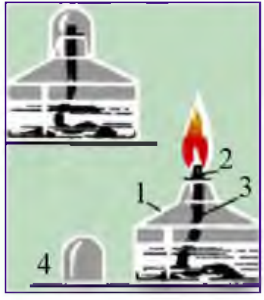
\includegraphics[width=0.86\linewidth]{rasmlar/darslik/d_spirt_lampa.png}\end{center}

\noindent\begin{tabular}{@{}p{0.47\linewidth}@{}p{0.47\linewidth}@{}}
A)~\textsl{metall disk} & B)~\textsl{qalpoqcha} \\
C)~\textsl{shtativ} & D)~\textsl{pilik} \\
\end{tabular}\par
\vspace{4pt}
\noindent\textbf{31.} Ba\textsuperscript{2+} ionini aniqlash uchun qaysi reagent mos va qanday belgi kuzatiladi?
\noindent A)~\textsl{NaOH: qo`ng`ir cho`kma (Fe(OH)\textsubscript{3})}\par
\noindent B)~\textsl{H\textsubscript{2}SO\textsubscript{4}: oq cho`kma (BaSO\textsubscript{4}), HCl da erimaydi}\par
\noindent C)~\textsl{BaCl\textsubscript{2}: oq cho`kma (BaSO\textsubscript{4}), HCl da erimaydi}\par
\noindent D)~\textsl{NaOH: oq-yashil cho`kma (Fe(OH)\textsubscript{2})}\par
\vspace{4pt}
\noindent\textbf{32.} 300 g 10\% li eritma tayyorlash uchun 80\% li eritmadan necha gramm olish kerak (qolgani suv)?

\noindent A)~\textsl{262,5} \hfill B)~\textsl{30} \hfill C)~\textsl{37,5} \hfill D)~\textsl{75   ---}\par
\vspace{4pt}
\end{multicols}
\medskip
\noindent\setlength{\fboxsep}{0pt}\fbox{\begin{tabular}{p{0.74\linewidth}|p{0.2\linewidth}}
\parbox[t]{0.72\linewidth}{\vspace{3pt}\textbf{Topshiriqlar (33--35) va javob variant (A--F)larini o`zaro to`g`ri moslashtiring.} CuO va Fe\textsubscript{2}O\textsubscript{3} dan iborat 12 g aralashma qizdirilib, H\textsubscript{2} oqimida to`liq qaytarildi; qoldiq (metallar) massasi 8,8 g.
\vspace{3pt}} & \parbox[t]{0.19\linewidth}{\vspace{3pt}A~\textsl{1,8}\\[3pt]
B~\textsl{3,6}\\[3pt]
C~\textsl{5,4}\\[3pt]
D~\textsl{6}\\[3pt]
E~\textsl{5,38}\\[3pt]
F~\textsl{4}}\\ \hline
\parbox[t]{0.72\linewidth}{\vspace{2pt}\textbf{33. Aralashmadagi CuO massasini (g) aniqlang.}\vspace{2pt}} & \\ \hline
\parbox[t]{0.72\linewidth}{\vspace{2pt}\textbf{34. Qaytarish uchun (20\% ortiqcha olingan) sarflangan H\textsubscript{2} hajmini (l, n.sh.) aniqlang.}\vspace{2pt}} & \\ \hline
\parbox[t]{0.72\linewidth}{\vspace{2pt}\textbf{35. Qaytarish natijasida hosil bo`lgan suv massasini (g) aniqlang.}\vspace{2pt}} & 
\end{tabular}}
\par\bigskip
\noindent\textbf{36.} FeSO\textsubscript{4} + KMnO\textsubscript{4} + H\textsubscript{2}SO\textsubscript{4} $\to$ Fe\textsubscript{2}(SO\textsubscript{4})\textsubscript{3} + MnSO\textsubscript{4} + K\textsubscript{2}SO\textsubscript{4} + H\textsubscript{2}O reaksiya tenglamasini tenglang. Reagentlar (chap qism) koeffitsiyentlari \textbf{yig`indisini toping.}
\javob
\noindent\textbf{37.} 6,5 g Zn reaksiyaga kirishdi (Zn + 2HCl $\to$ ZnCl\textsubscript{2} + H\textsubscript{2}). Ajralgan H\textsubscript{2} \textbf{hajmini (l, n.sh.) hisoblang} (unum 75\%).
\javob
\noindent\textbf{38.} Alyuminiy (0,1 mol) va kalsiy (0,1 mol) aralashmasi mo`l xlorid kislotada eritildi. Ajralgan vodorodning \textbf{hajmini (l, n.sh.) aniqlang.}
\javob
\noindent\textbf{39.} Etilatsetat va metilatsetat dan iborat 16,2 g aralashma mo`l NaOH eritmasi bilan to`liq gidrolizlandi. Hosil bo`lgan spirtlar umumiy \textbf{massasini (g) toping.}
\javob
\noindent\textbf{40.} 12 g sirka kislota va 13,8 g etanol dan 75\% unum bilan murakkab efir olindi. Efir \textbf{massasini (g) toping.}
\javob
\par\bigskip\begin{center}\textbf{\fontsize{13}{15}\selectfont YOZMA ISH}\end{center}
\noindent\textbf{41.} \textbf{Topshiriqni bajarish jarayonida barcha reaksiya tenglamalarini yozing. Miqdoriy va arifmetik hisoblashlarni (unga asos bo`lgan usul yoki formulani ko`rsatgan holda) uzviy ketma-ketlikda bajaring.}\par\smallskip
CuSO\textsubscript{4}$\cdot$5H\textsubscript{2}O va Na\textsubscript{2}SO\textsubscript{4}$\cdot$10H\textsubscript{2}O dan iborat 89,4 g aralashma 300 g suvda eritildi. Eritma inert elektrodlar yordamida 5 A tok kuchi bilan 3860 s elektroliz qilindi; shu vaqt tugaganda eritmadagi Cu\textsuperscript{2+} ionlari to`liq tugagan edi.\par
\noindent 1)Aralashmadagi kristallogidratlarning massalarini (g) aniqlang.\par
\noindent 2)Dastlabki eritmada CuSO\textsubscript{4} va Na\textsubscript{2}SO\textsubscript{4} ning massa ulushlarini (\%) toping. Elektroliz davomida o`tgan zaryadni (C) ham hisoblang.\par
\noindent 3)Anodda ajralgan gazning hajmini (l, n.sh.) va elektroliz tugagandan keyingi eritma massasini (g) aniqlang.\par
\noindent 4)Elektroliz tugagach eritmadagi H\textsubscript{2}SO\textsubscript{4} va Na\textsubscript{2}SO\textsubscript{4} ning massa ulushlarini (\%) hisoblang. Dastlabki CuSO\textsubscript{4} ning massasini (g) ham hisoblang.\par
\noindent 5)Shu eritmani to`liq neytrallash uchun zichligi 1,22 g/ml bo`lgan 20\% li NaOH eritmasidan necha ml kerak? Agar tok kuchi 2 marta oshirilsa, xuddi shu miqdor Cu ajralishi uchun necha sekund kerak bo`ladi?\par
\diqqat{Mazkur topshiriq kengaytirilgan javobni talab etib, uning yechilish usuli va shu usul asosidagi barcha hisoblash amallari javoblar varaqasida aks etishi lozim.}
\noindent\textbf{42.} Reaksiya tenglamalarini tugallang va tenglang. Hosil bo`lgan organik moddalarning tuzilish formulalarini yozing va ularni nomlang.\par
\noindent 1)CH\textsubscript{3}--CH(OH)--CH\textsubscript{3} + CuO $\xrightarrow{\text{t}}$\par
\noindent 2)CH\textsubscript{3}COOCH\textsubscript{3} + NaOH $\xrightarrow{\text{t}}$\par
\noindent 3)C\textsubscript{6}H\textsubscript{12}O\textsubscript{6} $\xrightarrow{\text{spirtli bijg`ish}}$\par
\noindent 4)CH\textsubscript{3}--C$\equiv$CH + H\textsubscript{2}O $\xrightarrow{\text{Hg\textsuperscript{2+}}}$\par
\noindent 5)3C\textsubscript{2}H\textsubscript{2} $\xrightarrow{\text{C, t}}$\par
\noindent 6)C\textsubscript{6}H\textsubscript{6} + HNO\textsubscript{3} $\xrightarrow{\text{H\textsubscript{2}SO\textsubscript{4}}}$\par
\noindent 7)n CH\textsubscript{2}=CH--CH=CH\textsubscript{2} $\to$\par
\diqqat{Mazkur topshiriq kengaytirilgan javobni talab etib, uning yechilish usuli va shu usul asosidagi barcha hisoblash amallari javoblar varaqasida aks etishi lozim.}
\noindent\textbf{43.} \textbf{Topshiriqni bajarish jarayonida barcha reaksiya tenglamalarini yozing. Miqdoriy va arifmetik hisoblashlarni (unga asos bo`lgan usul yoki formulani ko`rsatgan holda) uzviy ketma-ketlikda bajaring.}\par\smallskip
NaBr va NaI dan iborat 17,8 g aralashma suvda eritilib, mo`l xlor o`tkazildi. Eritma bug`latilib, qoldiq quritilganda uning massasi 8,78 g bo`ldi.\par
\noindent 1)Reaksiya tenglamalarini yozing. Aralashmadagi NaBr va NaI massalarini (g) toping.\par
\noindent 2)Sarflangan xlor hajmini (l, n.sh.) hisoblang. Hosil bo`lgan NaCl miqdorini (mol) ham toping.\par
\noindent 3)Ajralgan brom va yodning massalarini (g) toping.\par
\noindent 4)Dastlabki aralashma eritmasiga mo`l AgNO\textsubscript{3} qo`shilganda hosil bo`ladigan cho`kmalar massasini (g) aniqlang.\par
\noindent 5)Ajralgan brom va yod aralashmasida bromning massa ulushini (\%) toping.\par
\diqqat{Mazkur topshiriq kengaytirilgan javobni talab etib, uning yechilish usuli va shu usul asosidagi barcha hisoblash amallari javoblar varaqasida aks etishi lozim.}
\newpage
\noindent\textbf{\fontsize{13}{15}\selectfont Nazorat testi}\ \textit{$\cdot$ 6-variant}\hfill \textbf{Javoblar kaliti}\par\smallskip\hrule\smallskip
\textit{Faqat o`qituvchi uchun.}\par\medskip
\noindent\textbf{1--32-savollar}\par\smallskip
\noindent\begin{tabular}{|c|c|c|c|c|c|c|c|c|c|c|c|c|c|c|c|}\hline
\textbf{1} & \textbf{2} & \textbf{3} & \textbf{4} & \textbf{5} & \textbf{6} & \textbf{7} & \textbf{8} & \textbf{9} & \textbf{10} & \textbf{11} & \textbf{12} & \textbf{13} & \textbf{14} & \textbf{15} & \textbf{16}\\\hline
\textsl{C} & \textsl{D} & \textsl{A} & \textsl{D} & \textsl{B} & \textsl{B} & \textsl{A} & \textsl{B} & \textsl{D} & \textsl{D} & \textsl{D} & \textsl{B} & \textsl{A} & \textsl{C} & \textsl{C} & \textsl{D}\\\hline
\textbf{17} & \textbf{18} & \textbf{19} & \textbf{20} & \textbf{21} & \textbf{22} & \textbf{23} & \textbf{24} & \textbf{25} & \textbf{26} & \textbf{27} & \textbf{28} & \textbf{29} & \textbf{30} & \textbf{31} & \textbf{32}\\\hline
\textsl{A} & \textsl{C} & \textsl{A} & \textsl{C} & \textsl{C} & \textsl{A} & \textsl{A} & \textsl{C} & \textsl{D} & \textsl{B} & \textsl{B} & \textsl{B} & \textsl{A} & \textsl{D} & \textsl{B} & \textsl{C}\\\hline
\end{tabular}\par\medskip
\noindent\textbf{33--35-savollar}\par\smallskip
\noindent\begin{tabular}{|c|c|c|}\hline \textbf{No} & \textbf{Javob} & \textbf{Qiymat}\\\hline
33 & \textsl{F} & 4\\\hline
34 & \textsl{E} & 5,38\\\hline
35 & \textsl{B} & 3,6\\\hline
\end{tabular}\par\medskip
\noindent\textbf{36--40-savollar}\par\smallskip
\noindent\begin{tabular}{|c|c|}\hline \textbf{No} & \textbf{To`g`ri javob}\\\hline
36 & 20\\\hline
37 & 1,68\\\hline
38 & 5,6\\\hline
39 & 7,8\\\hline
40 & 13,2\\\hline
\end{tabular}\par\medskip
\noindent\textbf{41--43-topshiriqlar: qisqa yechim}\par\smallskip
\noindent\textbf{41-topshiriq.}\par
\noindent 1) Q = 5$\cdot$3860 = 19300 C = 0,2 mol e\textsuperscript{$-$}; Cu\textsuperscript{2+} + 2e\textsuperscript{$-$} $\to$ Cu: n(Cu\textsuperscript{2+}) = 0,1 mol $\to$ CuSO\textsubscript{4}$\cdot$5H\textsubscript{2}O \textbf{25 g}; Na\textsubscript{2}SO\textsubscript{4}$\cdot$10H\textsubscript{2}O = 89,4 $-$ 25 = \textbf{64,4 g} (0,2 mol)\par
\noindent 2) CuSO\textsubscript{4} 16 g; Na\textsubscript{2}SO\textsubscript{4} 28,4 g; eritma 389,4 g $\to$ \textbf{4,11\%} va \textbf{7,29\%}; Q = 5$\cdot$3860 = \textbf{19300 C}\par
\noindent 3) Anod: 2H\textsubscript{2}O $-$ 4e\textsuperscript{$-$} $\to$ O\textsubscript{2} + 4H\textsuperscript{+}: n(O\textsubscript{2}) = 0,05 mol $\to$ \textbf{1,12 l}; eritma: 389,4 $-$ 6,4 (Cu) $-$ 1,6 (O\textsubscript{2}) = \textbf{381,4 g}\par
\noindent 4) 2CuSO\textsubscript{4} + 2H\textsubscript{2}O $\to$ 2Cu + O\textsubscript{2} + 2H\textsubscript{2}SO\textsubscript{4}: H\textsubscript{2}SO\textsubscript{4} 0,1 mol = 9,8 g $\to$ \textbf{2,57\%}; Na\textsubscript{2}SO\textsubscript{4} 28,4 g $\to$ \textbf{7,45\%}; m(CuSO\textsubscript{4}) = 0,1$\cdot$160 = \textbf{16 g}\par
\noindent 5) H\textsubscript{2}SO\textsubscript{4} + 2NaOH $\to$ Na\textsubscript{2}SO\textsubscript{4} + 2H\textsubscript{2}O: NaOH 0,2 mol = 8 g; eritma 40 g; \textit{V} = 40/1,22 = \textbf{32,8 ml}; t = 3860/2 = \textbf{1930 s}\par
\noindent Jami: M 15 + A 10 = 25 ball.\par
\noindent\textbf{42-topshiriq.}\par
\noindent 1) CH\textsubscript{3}--CH(OH)--CH\textsubscript{3} + CuO $\xrightarrow{\text{t}}$ CH\textsubscript{3}COCH\textsubscript{3} + Cu + H\textsubscript{2}O --- propanon (4 ball)\par
\noindent 2) CH\textsubscript{3}COOCH\textsubscript{3} + NaOH $\xrightarrow{\text{t}}$ CH\textsubscript{3}COONa + CH\textsubscript{3}OH --- natriy atsetat va metanol (4 ball)\par
\noindent 3) C\textsubscript{6}H\textsubscript{12}O\textsubscript{6} $\xrightarrow{\text{spirtli bijg`ish}}$ 2C\textsubscript{2}H\textsubscript{5}OH + 2CO\textsubscript{2} --- etanol (3 ball)\par
\noindent 4) CH\textsubscript{3}--C$\equiv$CH + H\textsubscript{2}O $\xrightarrow{\text{Hg\textsuperscript{2+}}}$ CH\textsubscript{3}COCH\textsubscript{3} --- propanon (aseton) (3 ball)\par
\noindent 5) 3C\textsubscript{2}H\textsubscript{2} $\xrightarrow{\text{C, t}}$ C\textsubscript{6}H\textsubscript{6} --- benzol (4 ball)\par
\noindent 6) C\textsubscript{6}H\textsubscript{6} + HNO\textsubscript{3} $\xrightarrow{\text{H\textsubscript{2}SO\textsubscript{4}}}$ C\textsubscript{6}H\textsubscript{5}NO\textsubscript{2} + H\textsubscript{2}O --- nitrobenzol (3 ball)\par
\noindent 7) n CH\textsubscript{2}=CH--CH=CH\textsubscript{2} $\to$ (--CH\textsubscript{2}--CH=CH--CH\textsubscript{2}--)n --- polibutadiyen (4 ball)\par
\noindent Jami 25 ball.\par
\noindent\textbf{43-topshiriq.}\par
\noindent 1) 103x + 150y = 17,8; 58,5(x + y) = 8,78 $\to$ n(NaBr) = 0,1 mol (\textbf{10,3 g}), n(NaI) = 0,05 mol (\textbf{7,5 g})\par
\noindent 2) 2NaBr + Cl\textsubscript{2} $\to$ 2NaCl + Br\textsubscript{2}; 2NaI + Cl\textsubscript{2} $\to$ 2NaCl + I\textsubscript{2}: n(Cl\textsubscript{2}) = (x+y)/2 = 0,075 mol $\to$ \textbf{1,68 l}; n(NaCl) = 0,1 + 0,05 = \textbf{0,15 mol}\par
\noindent 3) Br\textsubscript{2}: \textbf{8 g}; I\textsubscript{2}: \textbf{6,35 g}\par
\noindent 4) AgBr: 0,1$\cdot$188 = 18,8 g; AgI: 0,05$\cdot$235 = 11,75 g; jami \textbf{30,55 g}\par
\noindent 5) $\omega$(Br\textsubscript{2}) = 8/(8 + 6,35) = \textbf{55,7\%}\par
\noindent Jami: M 15 + A 10 = 25 ball.\par
\par\bigskip\noindent\textbf{Mavzular taqsimoti}\par\smallskip
{\small\noindent\begin{longtable}{|c|p{7.2cm}|p{5.4cm}|c|}\hline \textbf{No} & \textbf{Mavzu} & \textbf{Tekshiriladigan ko`nikma} & \textbf{Ball}\\\hline
1 & 8-sinf; Tirkashev II bob (kimyoviy bog`lanish) & Bilim va tushunish & 1\\\hline
2 & 8-sinf (Gey-Lyussak, Avogadro) & Hisoblash va masala yechish & 1\\\hline
3 & Tirkashev VI bob (termokimyo, grafik) & Grafik tahlili & 1\\\hline
4 & 10-sinf \S{}17 (gibridlanish); Abdusamatov & Bilim va tushunish & 1\\\hline
5 & Tirkashev \textit{V} bob (OQR, jadval) & Jadval tahlili & 1\\\hline
6 & 8-sinf (Gey-Lyussak qonuni) & Hisoblash va masala yechish & 1\\\hline
7 & 11-sinf 8-bob; Tirkashev \textit{V} bob (elektroliz) & Bilim va tushunish & 1\\\hline
8 & 11-sinf (kovalent bog` turlari) & Rasm bo`yicha tahlil & 1\\\hline
9 & Tirkashev \textit{V} bob (kuchlanish qatori, jadval) & Jadval tahlili & 1\\\hline
10 & 11-sinf (ekvivalentlar qonuni) & Hisoblash va masala yechish & 1\\\hline
11 & Tirkashev I bob; 8-sinf (izoelektron) & Bilim va tushunish & 1\\\hline
12 & Tirkashev I bob; 8-sinf (elektron konfiguratsiya) & Bilim va tushunish & 1\\\hline
13 & 8-sinf; Tirkashev VI bob & Hisoblash va masala yechish & 1\\\hline
14 & 9-sinf; Tashev (anorganik birikmalar xossalari) & Bilim va tushunish & 1\\\hline
15 & Tashev (nitratlar termik parchalanishi) & Hisoblash va masala yechish & 1\\\hline
16 & 9-sinf (uglerod (IV) oksid) & Hisoblash va masala yechish & 1\\\hline
17 & 9-sinf; Tirkashev (galogenlar, hisob) & Hisoblash va masala yechish & 1\\\hline
18 & 9-sinf (ishqoriy metallar) & Hisoblash va masala yechish & 1\\\hline
19 & 9-sinf & Hisoblash va masala yechish & 1\\\hline
20 & 10-sinf (nomenklatura \S{}6, \S{}11, \S{}20, \S{}24--26) & Bilim va tushunish & 1\\\hline
21 & 10-sinf (mavzuga oid paragraflar); Abdusamatov & Bilim va tushunish & 1\\\hline
22 & 10-sinf \S{}15; Abdusamatov & Hisoblash va masala yechish & 1\\\hline
23 & 10-sinf (spirt, hisob) & Hisoblash va masala yechish & 1\\\hline
24 & 10-sinf \S{}24; \S{}26; \S{}30 (kumush ko`zgu) & Hisoblash va masala yechish & 1\\\hline
25 & 10-sinf (mavzuga oid paragraflar); Abdusamatov & Bilim va tushunish & 1\\\hline
26 & 10-sinf \S{}29 (yog`larni gidrogenlash) & Hisoblash va masala yechish & 1\\\hline
27 & 10-sinf (mavzuga oid paragraflar); Abdusamatov & Bilim va tushunish & 1\\\hline
28 & 10-sinf (ikki bosqichli hisob) & Hisoblash va masala yechish & 1\\\hline
29 & 10-sinf (pol, hisob) & Hisoblash va masala yechish & 1\\\hline
30 & 7-sinf (laboratoriya jihozlari, 3-rasm) & Rasm bo`yicha tahlil & 1\\\hline
31 & 9-sinf (sifat reaksiyalar) & Bilim va tushunish & 1\\\hline
32 & Tirkashev III bob (eritma tayyorlash) & Hisoblash va masala yechish & 1\\\hline
33--35 & Aralash masala (moslashtirish) & Ko`p bosqichli hisob & 3\\\hline
36--40 & Qisqa javobli masalalar & Hisoblash & 5\\\hline
41--43 & Yozma ish & Usul va hisob (M, A) & 75\\\hline
\end{longtable}}
\end{document}
